Mariella tiene bloques de plástico de igual tamaño y arma una torre con todos sus bloques como se observa en la Figura \ref{fig:bloques_plastico}:
Si Mariella decide completar la torre de tal forma que al final tenga 15 filas,

\textbf{¿cuántos bloques necesitará en total?}\\

\begin{minipage}{0.35\textwidth}
    \begin{figure}[H]
        \centering
        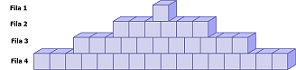
\includegraphics[width=0.95\linewidth]{../images/57c79607ac0a75446759bf7de89522cf0cbcea57}
        \caption{Ilustración de los bloques de plástico}
        \label{fig:bloques_plastico}
    \end{figure}
\end{minipage}\hfill
\begin{minipage}{0.6\textwidth}
    \begin{solutionbox}{5cm}
        Ya que la regla de recurrencia es:
        \[a_n=5(n-1)+1\]%
        entonces,
        \[a_{15}=5(15-1)+1=5(14)+1=71\]%
        y,
        \[s_{15}=\dfrac{15(a_1+a_{15})}{2}=\dfrac{32(1+71)}{2}=1152\]
    \end{solutionbox}
\end{minipage}




